\documentclass[a4paper,12pt]{article}
\usepackage{amsmath,amsfonts,amsthm,amscd,amssymb,latexsym}%,eufrak}
%%%%%%%%%%%%%
\usepackage{caption}
\usepackage{subcaption}
\usepackage{enumerate,graphicx,psfrag}%,subfigure}%,jchangebar,oldgerm}
\usepackage[mathscr]{eucal}
\usepackage[usenames]{color}
\usepackage{url}
\usepackage[shortlabels]{enumitem}
\usepackage{comment}
%\usepackage[utf8]{inputenc}
\usepackage[T1]{fontenc}
\usepackage{showkeys}
\usepackage{wrapfig}
\usepackage{lscape}
\usepackage{rotating}
\usepackage{xr}
%%%%%%%%%
\sloppy
%%%%%%%%%%%%%%%%%%%%%%%
\title{The subgroup membership problem in amalgamated products of 
finitely generated free groups
}
\author{Andrew J. Duncan, Elizaveta Frenkel}

\renewcommand{\a}{\alpha }
\renewcommand{\b}{\beta }
\newcommand{\G}{\Gamma }
\newcommand{\g}{\gamma }
\newcommand{\D}{\Delta }
\renewcommand{\d}{\delta }
%\def\vd{\vardelta}
\newcommand{\ep}{\epsilon }
\newcommand{\e}{\varepsilon }
\newcommand{\z}{\zeta }
%\eta
\renewcommand{\th}{\theta }
\newcommand{\T}{\Theta }
\renewcommand{\i}{\iota }
\renewcommand{\k}{\kappa }
\renewcommand{\l}{\lambda }
\renewcommand{\L}{\Lambda }
%\mu
%\nu
%\xi
%omicron
%\pi
\renewcommand{\r}{\rho }
\newcommand{\s}{\sigma }
\renewcommand{\S}{\Sigma }
\renewcommand{\t}{\tau }
\newcommand{\up}{\upsilon }
\newcommand{\U}{\Upsilon }
%\phi
\newcommand{\x}{\chi }
%\psi
\newcommand{\W}{\Omega }
\newcommand{\w}{\omega }
%%%%%%%%%%%%%%%%%%%%%%%%%%%%%%%
%%%%%%%%%%%%%%%%%%%%%%%%%%%%%
\newcommand{\pd}{\partial}
\newcommand{\wht}{\widehat}
%\newcommand{\cC}{{\mathcal C}}
%\newcommand{\cdim}{\texttt{cdim}}
\newcommand{\fC}{{\textswab C}}
\newenvironment{ef}{\noindent\color{blue} \bf EF: }{}
%
\newcommand{\cA}{{\cal{A}}}
\newcommand{\cD}{{\cal{D}}}
\newcommand{\cF}{{\cal{F}}}
\newcommand{\cH}{{\cal{H}}}
\newcommand{\cJ}{{\cal{J}}}
\newcommand{\cK}{{\cal{K}}}
\newcommand{\cP}{{\cal{P}}}
\newcommand{\cQ}{{\cal{Q}}}
\newcommand{\cR}{{\cal{R}}}
\newcommand{\cS}{{\cal{S}}}
\newcommand{\cV}{{\cal{V}}}
\newcommand{\cW}{{\cal{W}}}
%\newcommand{\GG}{\ensuremath{\mathbb{G}}}
\newcommand{\pp}{\mathbf{p}}
%%%%%%%%%%%%%%%%%%%%%%%%%%%%%%
\newcommand{\nul}{\emptyset }
\newcommand{\vim}{\nu\textrm{-im}}
%%%%%%%%%%%%%%%%%%%%%%%%%%%%%%
\newtheorem{theorem}{Theorem}[section]
\newtheorem{lemma}[theorem]{Lemma}
\newtheorem{corollary}[theorem]{Corollary}
\newtheorem{proposition}[theorem]{Proposition}
\newtheorem{axiom}[theorem]{Axiom}
\newtheorem{definition}[theorem]{Definition}
\newtheorem*{defn*}{Definition}
\newtheorem{conjecture}[theorem]{Conjecture}
%cvs -d :pserver:najd2@cvs.mas.ncl.ac.uk:/CVS/najd2
\newtheorem{exam}[theorem]{Example}
%\newtheorem{comment}[theorem]{Comment}
%
%
\newenvironment{example}{\begin{exam} \rm}{\end{exam}}
%
%
%
\newtheorem{remk}[theorem]{Remark}
\newenvironment{remark}{\begin{remk} \rm}{\end{remk}}
%
%%%%%%%%%%%%
\numberwithin{equation}{section}
\numberwithin{figure}{section}
%%%%%%%%%%%%%%%%%%%%
\newcommand{\Loop}{\operatorname{Loop}}
\newcommand{\Iso}{\operatorname{Isom}}
\newcommand{\Aut}{\operatorname{Aut}}
%%%%%%%%%%%%%%%%%%%
\renewcommand{\AA}{\ensuremath{\mathbb{A}}}
\newcommand{\ZZ}{\ensuremath{\mathbb{Z}}}
\newcommand{\QQ}{\ensuremath{\mathbb{Q}}}
\newcommand{\RR}{\ensuremath{\mathbb{R}}}
\newcommand{\NN}{\ensuremath{\mathbb{N}}}
\newcommand{\CC}{\ensuremath{\mathbb{C}}}
\newcommand{\FF}{\ensuremath{\mathbb{F}}}
%\renewcommand{\ker}{\verb"Ker"}
\newcommand{\cC}{\mathcal{C}}
\renewcommand{\cF}{\mathcal{F}}
\newcommand{\cO}{\mathcal{O}}
\renewcommand{\cS}{\mathcal{S}}
\newcommand{\cT}{\mathcal{T}}
\newcommand{\la}{\langle}
\newcommand{\ra}{\rangle}
%\newcommand{\BA}{\ensuremath{\mathbb{A}}}
%%%%%%%%%%%%%%%%%%%%%%%%%%%%%%%%%%%%%%
\newcommand{\maps}{\rightarrow}
\newcommand{\ov}[1]{\overline{#1}}
\newcommand{\bs}{\backslash}
%%%%%%%%%%%%%%%%%%%%%%%%%%%%%%%
\newcommand{\be}{\begin{enumerate}}
\newcommand{\ee}{\end{enumerate}}
\newcommand{\bd}{\begin{description}}
\newcommand{\ed}{\end{description}}
\newcommand{\biz}{\begin{itemize}}
\newcommand{\eiz}{\end{itemize}}
%%%%%%%%%%%%%%%%%%%%%%%%%%%%%%%%%%%
%
\newenvironment{ajd1}{\noindent\color{red} AJD }{}
\newcommand{\ajd}[1]{\begin{ajd1} #1 \end{ajd1}}
%
\newenvironment{bl}{\noindent\color{blue} EF }{}
\newcommand{\li}[1]{\begin{bl} #1 \end{bl}}
%\includecomment{comp}% to see environment comp
\excludecomment{comp}% to hide environment comp
%
\externaldocument{membership}
\begin{document}
Although $D=\{1\}\cup S$ is a set of double coset representatives, the 
representation of elements of $F$ in terms of double cosets $HDH$ is by 
no means unique; for example an element $h$ of $H$ may be expressed in
double coset normal form as  
as $a\cdot 1 \cdot b$,  for any $a,b\in H$ such that $ab=h$.  
Following \cite{FrenkelRemeslennikov13}, we use transversals for certain subgroups of $H$ to 
obtain unique double coset representations of elements of $F$. The subgroups
in question are the intersection $H\cap H^d$, where $d\in D$. 
 Using the  following lemma, and combining double coset representatives
with right transversals for these subgroups of $H$, we obtain the unique
representation we need. (There is no particular reason to choose right 
transversals here, and an analagous result holds for left transversals. However
the rewriting of elements of amalgamated products below depends on the choice
made here.)    
We write  $H_d=H\cap H^d$, whenever $H$ is a subgroup of a group $G$ and
$d\in G$. 
First we record a general property.  
\begin{lemma}\label{lem:dcrel}
Let $H$ be a subgroup of a group $G$ and let $D$ be a set of
double coset representatives for $H$. For each $d\in D$, let 
$T_d\subseteq H$ be a right transversal for the subgroup $H_d=H\cap H^d$ of $H$.
Then, given $g\in G$, there exist  unique $h\in H$, $d\in D$ and 
$t\in T_d$ such that  $g=hdt$. 
\end{lemma}
\begin{proof}
Let $g\in G$. As $D$ is a set of double coset representatives, there
exists a unique $d\in D$ such that $g\in HdH$, so it suffices to
show that there exist unique $h\in H$ and $t\in T_d$ such that 
$g=hdt$. Let $g=h_0dh_1$, where $h_i\in H$. Then there exist $a\in H_d$ 
and   $t\in T_d$ such that $h_1=at$. Then $a=d^{-1}bd$, for some $b\in H$,
so $g=h_0dh_1=h_0bdt\in HdT_d$. 

If $g$ can be written as  $g=h_0dt_0=h_1dt_1$, with $h_i\in H$ and 
$t_i\in T_d$, then $t_0t_1^{-1}=d^{-1}h_0^{-1}h_1d\in H_d$. As 
$T_d$ is a right transversal, this implies that $t_0=t_1$, so $h_0=h_1$. 
\end{proof}
\ajd{I am leaving this remark where it is, as I think it is 
easier to follow once the lemma has been established. What do you think?}
\begin{remark}
If $H^d=H$ then, in the notation of the lemma above, $T_d=1$ and 
every element of $HdH$ can be expressed uniquely in the form $hd$, 
with $h\in H$. In particular, if $H$ is normal in $G$ then $D$ is 
a right transversal for $H$ in $G$. On the other hand, if $H_d=1$ then
$T_d=H$ and $h_0dh'_0=h_1dh_1'$, with $h_i,h_i'\in H$, implies that 
$h_i=h'_i$, $i=1,2$. In particular, if $H$ is malnormal in $G$ then 
every element $g$ of $G\bs H$ can be written uniquely in the form 
$g=h_0dh_1$, where $h_i\in H$ and $d\in D$. 
\end{remark}   

Returning to the situation of Section \ref{sub:2cosetrepr}, 
where  $F=\FF(X)$, $H$ is a finitely generated subgroup of $F$ and $D=\{1\}\cup S^{(1)}\cup
S^{(2)}$ is a set of double coset representatives for $H$, 
we require transversals for the subgroups $H_d$ of $H$, for each $d\in D$. 
\begin{definition}\label{def:reltran}
Let $d\in D$ and let  $\cT_d'$ be a Schreier transversal for $H_d\le F$.
 Then we call $\cT_d=\cT_d'\cap H$ a 
\emph{relative  transversal for } $H_d$ in $H$. 
\end{definition}  
\ajd{
Say a bit more about Stallings foldings and Schreier transversals, 
somewhere, maybe?} 
\begin{proposition}[\emph{cf.} {\cite[Lemma 3.9]{FrenkelRemeslennikov13}}] \label{prop:reltran}
\be
\item\label{it:reltran1} 
Let $H$ be a finitely generated subgroup of $F$, let   $D=\{1\}\cup S^{(1)}\cup
S^{(2)}$ be a set of double coset representatives for $H$. Then for  each $d\in D$ the relative
transversal 
$\cT_d$ is a  transversal for $H_d$ in $H$.   
\item Every element $w$ of $F$ has a unique representation as 
$w=hdt$, where $h\in H$, $d\in D$ and $t\in \cT_d$. 
\ee
\end{proposition}
\begin{proof}
\be 
\item Let $g\in H$ and write $g=ht$,  where $h\in H_d$ and $t\in \cT_d'$.
As $g,h\in H$ it follows that $t\in \cT_D$, so $\cT_d$ is a transversal for 
$H_d$ in $H$.
\item This follows from statement \ref{it:reltran1} and Lemma 
\ref{lem:dcrel}. 
\ee
\end{proof}
\ajd{Now some discussion of relative transversal, which is not necessary, 
so should be deleted eventually or ....}
\li{This discussion contains a nice example, and to leave it here we can (try to) show that there is something which is not unique here, but we fix this problem with a help of your magic technic}
 Let $T$ be a spanning tree for $\G_H$ and let    $Y=\{y_1,\ldots, y_m\}$  be 
the corresponding set of  free generators for $H$. Let $Z=\{z_1,\ldots, z_m\}$ be
 a set disjoint from $F$ and let $\phi$ be the homomorphism from $\FF(Z)$ to $F$ induced by
$\phi(z_i)=y_i$. Then $\phi$ maps $\FF(Z)$ isomorphically to $H$. Let $\cF_Z$ be the rose of $\FF(Z)$ 
and let $\pi:\G_H \maps \cF_Z$ be the map which collapses each edge of $T$ to the vertex 
of $\cF_Z$ and maps  the interior of the edge of $\G_H\bs T$ corresponding to the generator $y_i$ homeomorphically to the interior of the   edge
(labelled) $z_i$ of $\cF_Z$. Then we relabel each edge $e$  of $\G_H$ as 
$x|v$, where $x\in X^{\pm 1}$ is the
original label of $e$, and 
\begin{itemize}
\item $v=1$ if $\pi(e)$ is the vertex of $\cF_Z$ and 
\item 
$v$ is the 
label of $\pi(e)$.  
\end{itemize}
In this way $\G_H$ becomes a transducer, which on
input a word $w\in F$ belonging to $H$, outputs a word $w'$ in $\FF(Z)$ such that $\phi(w')=w$. 
 The map $\pi_*$ of fundamental groups induced by $\pi$ is then equal to $\phi^{-1}$. 
For example, let $F=\FF(\{w,x,y\})$ and let $H$ be the subgroup
 generated by $xy^{-1}$, $yxy^{-2}$, $y^4$, $y^2xy$, $y^{-1}x$, 
$w^2$ and $wxyw^{-1}$, which we map to $z_1,\ldots ,z_7$ in the given order. 
Then we have the map of $\G_H$ to $\cF_Z$ shown in Figure \ref{fig:h} 
(where label $y|1$ is written just as $y$).
\begin{figure}
\begin{center}
\psfrag{pi}{$\pi$}
\psfrag{pia}{$\pi_a$}
\psfrag{piz}{$\pi_Z$}
\psfrag{rho}{$\rho$}
\psfrag{GH}{$\G_H$}
\psfrag{Gz}{$\G_a^Z$}
\psfrag{GHa}{$\G_{H_a}$}
\psfrag{Fz}{$\cF_Z$}
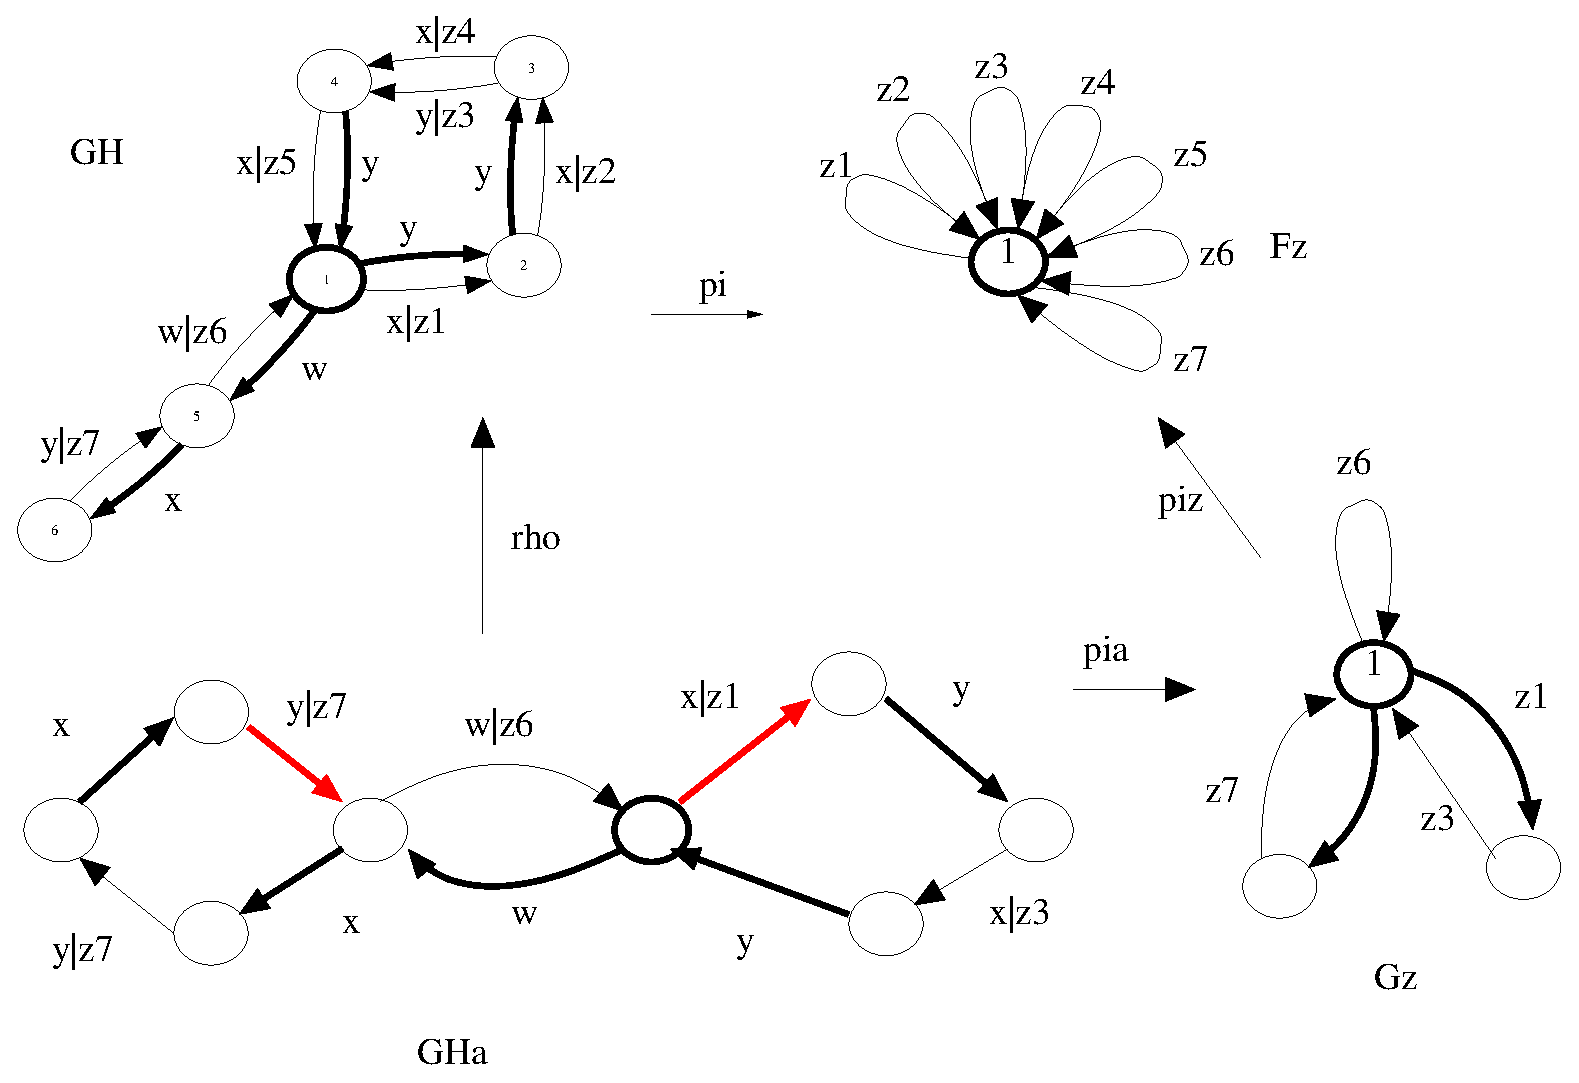
\includegraphics[scale=.5]{../python/genfold/hs.eps}
\end{center}
\caption{}\label{fig:h}
\end{figure}

Now let $a$ be the label of a path in $T$ ($a\neq 1$) and let $\t(a)$ be the final vertex of this
path. Let $\G_a'$ be the core of the connected component of $\G_H\times \G_H$ containing 
$(\t(a),1)$. Then 
 $w$ is the label of a reduced path in $\G_a'$ if and only if $w$ is both the 
label of a closed path in $\G_H$ based at $1$ and a closed path based at $\t(a)$. Hence 
$w$ is the label of a reduced path in $\G_a'$ if and only if $w\in H_a$. Thus, as it is
folded, and has no vertices of degree $1$, except possibly its root,  $\G_a'$ is the 
core of the universal cover of $H_a$; which is the Stallings folding of $H_a$. 
All this is completely standard, and I'm just being pedantic (and establishing notation).

Next, let $\rho:\G_{H_a} \maps \G_H$ be the canonical map (which is an immersion).
We use the same set of labels for edges of $\G_{H_a}$ as for $\G_H$; that is, if $\rho(e)$ is 
an oriented edge labelled $x|v$ then the label of $e$ is also $x|v$, for all edges $e$ of $\G_{H_a}$. 
%Then $\pi\circ \rho$ maps $\G_{H_a}$ to $\cF_Z$ by first mapping to 
%$\G_H$ and then shrinking edges; an edge $e$ is shrunk to 
%the vertex of $\cF_Z$ if its label is $x|1$, and has its interior mapped homeomorphically to
%the interior of the  edge of $\cF_Z$ labelled $z$, if it is labelled $x|z$.
Let $E_0$ be the set of edges of $\G_{H_a}$ labelled $x|1$, for some $x\in X$. Then the union
$T_a'$ of all edges in $E_0$ forms a subgraph of  $\G_{H_a}$ which I claim is a forest. The claim
holds because if $C$ is a non-trivial 
reduced closed path in $T_a'$ then it maps to a closed  path $C'$ in $T$ (since its 
edges all have label $x|1$) and, since the map $\rho$ is an immersion, $C'$ is also reduced, a
contradiction. Now add edges to $T_a'$ to form a spanning subtree $T_a$ of $\G_{H_a}$.  In the example in Figure \ref{fig:h} I have taken $a=w$ and 
the edges of $T_a'$ are bold black, while the edges added to form $T_a$ are
red. 

We can form a new graph $\G_a^Z$ from $\G_{H_a}$ by shrinking all edges with label $x|v$ such
that $x\in X$ and $v=1$ and then folding the resulting graph.  Let $\pi_a$ be the natural map from $\G_{H_a}$ to $\G_a^Z$.  I claim now that $\pi_a(T_a)$ is a spanning tree for $\G_a^Z$. To begin with,
$\pi_a(T_a)$ is a subgraph of $\G_a^Z$ containing every vertex (as $T_a$ contains every vertex
of $\G_{H_a}$). Suppose that $\pi_a(T_a)$ contains a closed reduced path. This is obtained from
a path in $T_a$ by shrinking edges: and so $T_a$ contains a closed reduced path, a contradiction.
Thus $\pi_a(T_a)$ is a tree as claimed. On the other hand, there is a map $\pi_Z:\G_a^Z\maps
\cF_Z$, mapping every edge of $\G_a^Z$ labelled $z$ to the unique edge of $\cF_Z$ labelled $z$,
for all $z\in Z$. Clearly (and we all know what that means) $\pi\circ \rho=\pi_Z\circ \pi_a$, 
so the image of $\pi_1(\G_a^Z)$ under the map $(\pi_Z)_*$ is equal to 
$(\pi\circ\rho)_*(\pi_1(\G_{H_a}))=\pi_*(H_a)=\phi^{-1}(H_a)$. This means that the
rank of $\pi_1(\G_a^Z)$ is greater than or equal the rank of $H_a$, and since it is at most
the number of edges outside the spanning tree $T_a$ of $\G_{H_a}$, which is equal the to 
the rank of $H_a$; the rank of $\pi_1(\G_a^Z)$ is equal to the rank of $H_a$. It follows
(by consideration of Euler characteristic) that no two edges of $\G_{H_a}\bs T_a$ are folded
together in the map $\pi_a$ from $\G_{H_a}$ to $\G_a^Z$ and that $\G_a^Z$ is the Stallings
folding for $\phi^{-1}(H_a)$. This is the conclusion that I want because now the spanning
tree for the Stallings folding $\G_a^Z$ of  $\phi^{-1}(H_a)$ is the image under $\pi_a$ of the 
spanning tree $T_a$ for $\G_{H_a}$. Moreover, edges of $\G_{H_a}$ outside the spanning tree $T_a$ map to edges
outside the spanning tree for $\G_a^Z$ (by consideration of rank).
This means that, if $w$ is the label of a path $p$ in $T_a$, 
from $1$ to some vertex
of $\G_{H_a}$, and simultaneously an element of $H$, then the path
$p$ is mapped by $\pi_a$ to a path in $\G_a^Z$ with label $\phi^{-1}(w)$. 
\li{comprehensible but not so clearly written...}


Now, let $\cT_a^X$ be the Schreier transversal for $H_a\le F$ obtained from
the spanning tree $T_a$ for $\G_{H_a}$. Let $\cT_a^Y=\cT_a^X\cap H$. Then $\cT_a^Y$ is
 a transversal for $H_a\le H$. From the above,  
 internal representives of the  transversal $\cT_a$ are mapped 
by $\phi^{-1}$ to labels of paths in  
in $T_a$. As $\phi^{-1}$ is an isomorphism $\phi^{-1}(\cT_a)$ is 
a transversal $S$ for  $\phi^{-1}(H_a)$ in $\FF(Z)$. Each exterior representative
of $\cT_a$ is mapped by $\pi_a$ to a path which represents an element
of this transversal $S$. Since $T_a$ is mapped by $\pi_a$ to a spanning
tree for $\G_a^Z$ it follows that all these paths end at vertices of the
cover of $\phi^{-1}(H_a)$ outside $\G_a^Z$. Hence exterior representatives
of $\cT_a$ are mapped to exterior representatives of the transversal
of $\phi^{-1}(H_a)$ corresponding to the tree $\pi_a(T_a)$. Thus $S$
is in fact a Schreier transversal.
 ($\cT_a^Y$ is not in general a Schreier transversal. For example
consider the representative $xyx^{-1}y^{-1}$. This is the product
of $xy^{-1}$ and $y^2x^{-1}y^{-1}$, which are both in $\cT_a$. However
the cancellation in forming their product means that, even if we 
restrict to generators $Y$ the transversal does not behave as it 
should with respect to prefixes.)
\ajd{End of bit about transversals -- to be deleted in due course.}
\li{(just in case we will this piece remains, we need to say what is interior and exterior representative.) }
 
To rewrite elements of $dH$ in the form $hdt$, where $h\in H$, 
$d\in D$ and $t\in \cT_d$ 
we shall fix the transversals $\cT_d$, for elements $d$ of $D$, and
then use the algorithm implicit in the proof of Lemma \ref{lem:reltran}
below. We shall use the following facts, the proofs of which
are left to the reader. \ajd{At least they will probably be deleted 
from  the final version.}
\begin{lemma}\label{lem:conjtran}
Let $K$ be a finitely generated subgroup of $F$ and let $T$ be
a transversal for $K$. Let $a\in F$ and let 
$a^{-1}T=\{w\in F:w=a^{-1}t, t\in T\}$ 
(so elements of $a^{-1}T$ are reduced words). 
  Then 
\be
\item $a^{-1}T$ is a transversal for $K^a$ and 
\item if $T$ is a Schreier transversal and $a\in T$ 
then $a^{-1}T$ is a Schreier  transversal for $K^a$.
\ee
\end{lemma}
\begin{proof}
\be
\item If $g\in F$ then $ag=kt$, for some $k\in K$ and $t\in T$, 
so $g=(a^{-1}ka)(a^{-1}t)\in K^aa^{-1}T$. Uniqueness of this representation
follows from the obvious computation.
\item Let $t\in T$. 
We may assume that we have $a=a_0\circ a_1$, $t=t_0\circ t_1$, where
$t_0=a_0$ and $a^{-1}t=a_1^{-1}\circ t_1$ (and possibly $a_0=1$ or $a_1=1$).  
%As $a,t\in T$ so are  $a_0$ and $t_0$.  
Every prefix of $a^{-1}t$ then has the form $a_1^{-1}t'$, for 
some prefix $t'$ of $t_1$, or the form $a'$, for some prefix $a'$ of 
$a_1^{-1}$.  If $t'$ is a prefix of $t_1$ then $t_0t'\in T$ and 
$a_1^{-1}t'=  a^{-1}t_0t'\in a^{-1}T$. If $a^{-1}=a'a''$ then 
$(a'')^{-1}$ is a prefix of $a$, so belongs to $T$, and $a'=a^{-1}(a'')^{-1}
\in a^{-1}T$. Hence, in all cases, every prefix of $a^{-1}t$ belongs
to $a^{-1}T$, which is therefore Schreier.
\ee
\end{proof}
\begin{lemma}\label{lem:reltran}
For each $d\in D$, there is a 
relative Schreier transversal $\cT_d$, for $H_d\le H$, and there is  
 an algorithm that, given $d\in D$ and a word $w \in F$ such that 
$w\in H$, outputs $a,t\in F$ such that $a\in H_d$, $t\in \cT_d$ and 
$w=_F at$. 
\end{lemma}
\begin{proof}
We may assume that we have constructed $\G_H$ and $\G_H\times \G_H$ and
that we have chosen  spanning trees for $\G_H$ and for 
each component of 
 $\G_H\times \G_H$. 
If $d=1$ then $H_d=H$ and $\cT_d=\{1\}$, so the algorithm 
%writes 
%$w$ as a word in the generators $Y$ (using the Stallings folding $\G_H$
% for $H$) and 
outputs $a=w$ and $t=1$.  
If $d\in S^{(1)}$ then no non-trivial element of $H^d$ is accepted 
by $\G_H$, so
$H\cap H^d=\{1\}$ and $\cT_d=H$. In this case the algorithm 
%writes $w$ as a word in the generators $Y$, using $\G_H$,  and 
outputs $a=1$, $t=w$. 

Assume then that $d\in S^{(2)}$, say $d=a_0a_1^{-1}$, where 
$a_0$ is a maximal $L_Q$-prefix and an $L_T$-prefix of $d$ and $a_1$ is in 
$L_T$. 
%%
In principle the algorithm  now constructs the 
Stallings folding for $H_d$ and then uses this to 
find the required expression for $w$ (in much the same 
way that the Stallings folding for $H$ is used to find double
coset representatives.) However, it turns out, as we show below, that
$\G_H\times \G_H$ contains the Stallings folding for the 
conjugate $H^{a_1}\cap H^{a_0}=H_d^{a_1}$ of $H_d$; and that 
the expression for $w$ can in fact be computed using this instead. 

To see this, let $u_i=\t(a_i)$, $i=0,1$. Then there exists
a path labelled $a_i$ from $1$ to $u_i$, in $\G_H$, for $i=1,2$.
 This implies in particular that, for 
all $\b,\g\in H$, there exists 
a closed path labelled $a_0^{-1}\b a_0$, based at 
$u_0$, and  a closed path labelled $a_1^{-1}\g a_1$, based at 
$u_1$. 

We have $c\in H_d$ if and only if there exists $b\in H$ such that
$a_1^{-1}ca_1=a_0^{-1}ba_0$. Thus, if $c\in H_d$ then 
 there exists a closed path
labelled $a_1^{-1}ca_1$ based at $(u_0,u_1)$ in $\G_H\times \G_H$. 
Conversely, if there is a closed path labelled $s$ based at 
$(u_0,u_1)$ then there are closed paths labelled 
$s$ based at $u_0$ and $u_1$ in $\G_H$. Hence 
$b=a_0sa_0^{-1}$ and $c=a_1sa_1^{-1}$ are in $H$, 
and satisfy $a_1^{-1}c a_1=s=a_0^{-1}ba_0$. Therefore $c \in H_d$. 
 Let $\G'_d$ be the component of $\G_H\times \G_H$
containing $(u_0,u_1)$ and let $T_d'$ be the spanning tree 
chosen for $\G_d'$. It follows from the above that the map
from $\pi_1(\G_d', (u_0,u_1))$ to $H_d$ sending $s$ to $a_1sa_1^{-1}$, is 
an isomorphism; and so  
$\pi_1(\G_d', (u_0,u_1))\cong H^{a_1}\cap H^{a_0}\le F$.
As $\G_d'$ is folded it is a subgraph of the cover
$\G_d^*$ corresponding to  $H^{a_1}\cap H^{a_0}$, and the spanning tree $T_d'$ for 
$\G_d'$ embeds in a spanning tree $T_d^*$ for $\G_d^*$. 
Note that, by definition of $S^{(2)}$, no non-trivial prefix of 
$a_1^{-1}$ is readable from $u_0$ in $\G_H$. This means no non-trivial
prefix of $a_1^{-1}$ is readable from $(u_0,u_1)$ in $\G_d'$. Therefore
$T_d^*$ contains a (unique) path  labelled $a_1$ ending
at the vertex $(u_0,u_1)$ of $\G_d'$, all edges of which lie 
outside $\G_d'$. 

The labels of paths in $T_d^*$, with inital vertex $(u_0,u_1)$,
 constitute 
a Schreier transversal $\cT_d'$ for $H^{a_1}\cap H^{a_0}$ in  $F$.
As $a_1^{-1}$ belongs to this Schreier transversal the set 
$\cT_d=a_1\cT_d'$ is (according to Lemma \ref{lem:conjtran}) 
a Schreier transversal for $a_1(H^{a_1}\cap H^{a_0})a_1^{-1}=H^d$ in $F$. 
 
Given $w\in F(X)$ such that $w\in H$, we require 
an expression $w=_F a t$, such that $a\in H_d$ and $t\in \cT_d$ 
(in which case $t\in \cT_d\cap H$). However, the graph $\G_d'$ 
 which we have constructed, enables us only to find an expression
$w=a't'$, where $a'\in H^{a_1}\cap H^{a_0}$ and $t'\in \cT_d'$. Therefore
we first replace $w$ with  
  $w'=a_1^{-1}w$ (as a reduced word).  
 Next find the maximal
prefix $f$ of $w' $ which is accepted by $\G_{d}'$ (with
start and final state $(u_0,u_1)$) say $w'=f\circ q$.
Let $g$ be the maximal
 prefix of $q$ which is readable by $\G_{d}'$; say $q=g\circ r$. Let 
$v=\t(g)$ and let $s=w(v)$, the label of the path from $(u_0,u_1)$ 
to $v$ in $T_d'$, the chosen spanning tree for $\G_d'$. 
Then $w'=fq=fgr=(fgs^{-1})(sr)$, with $h'=fgs^{-1}\in H^{a_1}\cap H^{a_0}$ 
and $t'=sr\in \cT_d'$. Hence 
$w=a_1w'=a_1 h' a_1^{-1}(a_1t')\in H_d \cT_d$. The algorithm outputs
 $a=  a_1 h' a_1^{-1}$ and $t=a_1t'$. 
\end{proof}
%%%%%%%%%
%% keeping this till the alternative is checked
%%%%%% 
\begin{comment}
assume that $H$ is freely generated by a set $Y=\{y_1,\ldots,
y_m\}$.  
Let $Z=\{z_1,\ldots ,z_m\}$ be a set disjoint from $F$ and 
let $\phi$ be the homomorphism from $\FF(Z)$ to $F$ induced by 
$\phi(z_i)=y_i$, $i=1,\ldots, m$.
\begin{definition}\label{def:reltran}
Let $d\in D$ and let $U_d=\phi^{-1}(H_d)$. Let $T_d^Z$ be a spanning tree
for the Stallings folding of $U_d$ and let $\cT_d^Z$ be the corresponding 
Schreier transversal, for $U_d$ in $\FF(Z)$. \ajd{The Schreier transversal
corresponding to a spanning tree of a Stallings folding needs to be
defined somewhere: probably not just here.} Then $\cT_d=\phi(\cT_d^Z)
\subseteq H$ is called a \emph{relative transversal for } $H_d$ in $H$. 
\end{definition}   
\begin{proposition}[\emph{cf.} {\cite[Lemma 3.9]{FrenkelRemeslennikov13}}] \label{prop:reltran}
\be
\item\label{it:reltran1} The set $\cT_d$ is a Schreier transversal for the subgroup 
$H_d$ of $\FF(Y)$. 
\item Every element $w$ of $F$ has a unique representation as 
$w=hdt$, where $h\in H$, $d\in D$ and $t\in \cT_d$. 
\ee
\end{proposition}
\begin{proof}
\be 
\item If $g\in \FF(Y)$ then $g=\phi(g')$, for some $g'\in \FF(Z)$, and 
$g'=ut'$, where $u\in U_d$ and $t'\in \cT_d^Z$. Thus $g=\phi(u)\phi(t')
\in H_d\cT_d$. Moreover, if $g=h_0t_0=h_1t_1$, with $h_i\in H_d$ and 
$t_i\in \cT_d$, then $\phi^{-1}(g)=\phi^{-1}(h_i)\phi^{-1}(t_i)$, $i=0,1$,
from which it follows that $t_0=t_1$ and $h_0=h_1$. Hence $\cT_d$ is 
a transversal for $H_d$. 

If $w\in \cT_d$ and $w=w_0\circ w_1$ then 
$\phi^{-1}(w)=\phi^{-1}(w_0)\circ \phi^{-1}(w_1)\in \cT^d_Z$, so $\phi^{-1}(w_0)
\in \cT_d^Z$ and hence $w_0\in \cT_d$; so $\cT_d$ is a Schreier 
transversal.
\item This follows from statement \ref{it:reltran1} and Lemma 
\ref{lem:dcrel}. 
\ee
\end{proof}
\begin{lemma}\label{lem:reltran}
There is an algorithm that, given $d\in D$ and a word $w \in F$ such that 
$w\in H$, outputs $a,t\in \FF(Y)$ such that $a\in H_d$, $t\in \cT_d$ and 
$w=_F ht$. 
\end{lemma}
\begin{proof}
If $d=1$ then $H_d=H$ and $\cT_d=\{1\}$, so the algorithm writes 
$w$ as a word in the generators $Y$ (using the Stallings folding $\G_H$
 for $H$) and outputs $a=w$ and $t=1$. 

If $d\in S^{(1)}$ then no non-trivial element of $H^d$ is accepted by $\G_H$, so
$H\cap H^d=\{1\}$ and $\cT_d=H$. In this case the algorithm writes
$w$ as a word in the generators $Y$ and outputs $a=1$, $t=w$. 

We may assume then that $d\in S^{(2)}$, say $d=a_0a_1^{-1}$, where 
$a_0$ is a maximal $L_Q$-prefix and an $L_T$-prefix of $d$ and $a_1$ is in 
$L_T$. Then $c\in H_d$ if and only if there exists $b\in H$ such that
$a_1^{-1}ca_1=a_0^{-1}ba_0$. Let $u_i=\t(a_i)$, $i=0,1$. Then there exists
a path labelled $a_i$ from $1$ to $u_i$, in $\G_H$, for $i=1,2$. Thus for
all $b,c\in H$ there exists,  in $\G_H$, 
a closed path labelled $a_0^{-1}ba_0$, based at 
$u_0$, and  a closed path labelled $a_1^{-1}ca_1$, based at 
$u_1$. 

If $a_1^{-1}ca_1=a_0^{-1}ba_0$ then there exists a closed path
labelled $a_1^{-1}ca_1$ based at $(u_0,u_1)$ in $\G_H\times \G_H$. 
Conversely, if there is a closed path labelled $s$ based at 
$(u_0,u_1)$ then, in $\G_H$,  there are closed paths labelled 
$s$ based at $u_0$ and $u_1$. Hence $h_i=a_isa_i^{-1}\in H$, for 
$i=0,1$,  and so $a_1^{-1}h_1 a_1=s=a_0^{-1}h_0a_0$. Hence $h_1
=a_1sa_1^{-1}\in H_d$. Let $\G'_d$ be the component of $\G_H\times \G_H$
containing $(u_0,u_1)$. It follows from the above that the map
from $\pi_1(\G_d', (u_0,u_1))$ to $H_d$ sending $s$ to $a_1sa_1^{-1}$, is 
an isomorphism. Hence we may construct $\G_{H_d}$ from $\G'_d$ by
attaching the terminal vertex of a path labelled $a_1$ to the 
vertex $(u_0,u_1)$ and folding the result. 
 
Now, given $w\in F(X)$ such that $w\in H$ we may find the maximal
prefix $f$ of $w$ which is accepted by $\G_{H_d}$, say $w=f\circ q$.
Now choose a spanning tree $T_d$ for $\G_{H_d}$. Let $g$ be the maximal
 prefix of $q$ which is readable by $\G_{H_d}$; say $q=g\circ r$. Let 
$v=\t(g)$ and let $s=w(v)$, the label of the path from $1$ to $v$ in $T_d$.
Then $w=fq=fgr=fgs^{-1}sr$, with $fgs^{-1}\in H_d$ and $sr\in \cT_d$.    
\ajd{This isn't quite complete, as in the definition we choose $\cT_d$ to
be the image of a Schreier transversal for $U_d\in \FF(Z)$, and this means
that we should choose a spanning tree for $\G_{H_d}$ which is the
image of a spanning tree for $\G_{U_d}$ and then construct the 
transversal from this tree. I'm leaving these details for another day.}
Then the algorithm outputs $a=fgs^{-1}$ and $t=sr$. Note that we 
can find expressions for these in terms of generators $Y$  with the
help of $\G_H$ and its output labels. 
\end{proof}
\end{comment}
%%%%%%%%%%%%%%%%%%%%
%%delete the above once the alternative is checked
%%%%%%%%
\subsection{Double coset normal forms in the free group}
If $w\in F$ then we say that a triple $(a,d,t)$ is the 
\emph{double coset normal form} of $w$ 
(with respect to $H$ and $D$, defined above) if $w=_F adt$, 
$a\in H$, $d \in D$ and $t\in \cT_d$, the relative transversal 
for $H_d\le H$. From Proposition \ref{prop:reltran} every element
of $F$ has a unique double coset normal form. When the meaning
is clear we shall drop the triple notation and write the
normal form $(a,d,t)$  as $adt$. 
In the light of the proof of  Proposition \ref{prop:dcreps} and  Lemma 
\ref{lem:reltran} there exists an
 algorithm to find the double coset normal form of an element of $F$. 
Algorithm I in  Sections \ref{sub:sum_algI} and  \ref{sub:alg1ex} carries out this process. The first part of
this  algorithm, in Section \ref{sub:sum_algI}, constructs the 
automata necessary for processing  with respect to a chosen
 subgroup $H$ of $F$. The next part of  the  algorithm in 
Section \ref{sub:alg1ex},  Steps \ref{it:alg1_1} to \ref{it:dc1},
following the proof of Proposition \ref{prop:dcreps},  
  takes  a word  $w\in F$ and finds an triple
$(h,d,h')$, where $h,h'\in H$, $d\in \{1\}\cup S^{(1)}\cup S^{(2)}$
and $w=_F hdh'$. If $d$ is in $\{1\}\cup S^{(1)}$ the algorithm
outputs this triple. Otherwise, the word $h'$ is rewritten, 
as in   
Lemma \ref{lem:reltran}, as $h'=gt$, where $g\in H_d$ and  $t\in \cT_d$.
As $g\in H_d$ there exists  and $g'\in H$ such that $g'=d^{-1}gd$ 
and so we have $w=hdh'=hdgt=hg'dt=adt$, where $a=hg'\in H$. The 
  algorithm outputs $(a,d,t)$. 

To see that the algorithm in Section \ref{sub:sum_algI} does give the 
required output, note first that if $w\in F$ belongs to a double
coset $HdH$, where $d\in \{1\}\cup S^{(1)}$, then Steps \ref{it:alg1_1} to
\ref{it:dc1} carry through the process implicit in the proof of 
Proposition \ref{prop:dcreps} and outputs $(a,b,c)$, where $b=d$, $a,c\in H$,
and $w=abc$. In this case the transversal $\cT_d=\{1\}$ and so 
$(a,b,c)$ is the double coset normal form of $w$. On the other hand
if $w=hdh'$, where $d$ is in $S^{(2)}$, then it follows from the 
proof of Proposition \ref{prop:dcreps}, that such (unique) 
$d$ is found in Step \ref{it:dc2}
of the algorithm. At this point 
$w=hpcy^{-1}\cdot yz^{-1}\cdot zc^{-1}t^{-1}g^{-1}$, with
 $hpcy^{-1}$ and $zc^{-1}t^{-1}g^{-1}$ in $H$ and $d=yz^{-1}\in D$. 
The next step is to find the representative of $zc^{-1}t^{-1}g^{-1}$ 
in $\cT_d$. As in the proof of Lemma \ref{lem:reltran} to do this
$\b'=zc^{-1}t^{-1}g^{-1}$  is replaced by $\b=z\b'= c^{-1}t^{-1}g^{-1}$.
Here $y=w(u_0)$ and $z=w(v_0)$, where $u_0=\t(p)$ and $v_0=\t(t)$.  
The component $\G_d$ of $\G_H\times \G_H$ 
containing the vertex $(u_0,v_0)$ is then
used to find an expression $\b=\b_0\circ \g_0\circ \g_1$, where $\b_0$
is the maximal prefix of $\b$ accepted by $A_d=(\G_d,(u_0,v_0))$ and $\g_0$ is
the maximal prefix of $\b_1$ readable by $A_d$. A spanning forest
$F_H$ for $\G_H\times \G_H$ has been computed by the algorithm of 
Section \ref{sub:sum_algI} and the component of this forest contained
in $\G_d$ is denoted $T_d$. The algorithm finds the label $\d$ of a path
from $(u_0,v_0)$ to $\t(\g_0)$ in $T_d$. As in the proof of Lemma 
\ref{lem:reltran}, $\b=(z\b_0\g_0\d^{-1}z^{-1})(z\d\g_0)$, with
$t=z\d\g_0\in \cT_d$ and $\b''=z\b_0\g_0\d^{-1}z^{-1}\in H_d$. The output
from the algorithm is then $(a,yz^{-1},t)$, where 
\[a=hpcy^{-1}(yz^{-1})\b''(yz^{-1})^{-1}
=hpcz^{-1}(z\b_0\g_0\d^{-1}z^{-1})zy^{-1} =hpc\b_0\g_0\d^{-1}y^{-1}.\]

\begin{example}\label{ex:f_1_again}
Consider the elements 
$f_1$ and $f_2$ of the free group $F_1$ of Example \ref{ex:f_1}. 
In that example we found  
\[f_1=hs_1(h^\prime)^{-1}=(h_2^{2}h_1) x_1x_3^3x_1(h_1^{-1}h_3^{-1})\in H_1S_1^{(1)}H_1,\]
with $s_1=x_1x_3^3x_1$ the double coset representative of $f_1$. 
As $s_1\in S_1^{(1)}$, as in the proof of Lemma \ref{lem:reltran}, 
$H_{s_1}=\{1\}$ and so $(h^\prime)^{-1}\in \cT_{s_1}$. Thus
$f_1$ has double coset normal form $(h, s_1, (h^\prime)^{-1})$.

We also found 
\[f_2=a yz^{-1} b=(h_3^{-1}h_2^{-1}) x_1^{-1}\]
with $a=h_3^{-1}h_2^{-1}$, $b=1$ and $s_2=yz^{-1}= x_1^{-1}\in S_1^{(2)}$ 
 the double coset representative of $f_2$. 
In this case $z=1$, so $H^z\cap H^y=H\cap H^y=H\cap H^{s_2}=H_{s_2}$. 
Furthermore, as $b=1$ we see immediately that $t=b=1$ and the
double coset normal form of $f_2$ is $(h_3^{-1}h_2^{-1}, x_1^{-1}, 1)$.
\end{example}

\begin{example}\label{ex:f_2_again}
Consider the element $f_1'$ of Example \ref{ex:f_2}. 
We found 
\[f_1^\prime=h yz^{-1} g^{-1},\]
where $h=h^\prime_3h_2^\prime$, $g^{-1}=h_2^\prime h_1^\prime$,  
$y=y_1$, $z=y_2^{-1}$ and $s_1'=yz^{-1}=y_1y_2\in S_2^{(2)}$ is the 
double coset representative of $f_1'$. In this case $s_1'$ corresponds
to the vertex $(3,2)$ of $\G_{H_2}\times \G_{H_2}$. As this is an 
isolated vertex it follows, as in the proof of Lemma \ref{lem:reltran},
that $H_{s_1'}=\{1\}$. Therefore $\cT_{s_1'}=H_2$ and the 
double coset normal form of $f_1'$ is 
$(h,s_1',g^{-1})$.  
\end{example}
\ajd{These two examples are typical, as subgroups of $F$ are generically
malnormal, and even when they are not 
double cosets representatives are generically of type 1 (aren't they; there
are only finitely many of type 2). Oh, but this may not be a sensible thing
to say, as what counts is the size of the dobule cosets $HdH$. Lisa,
you probably know how to say this?}
\begin{example}\label{ex:reltran}
\ajd{This is the same example as above, in the discussion of 
relative transversals} 
For example, let $F=\FF(\{a,b,c\})$ and let $H$ be the subgroup
 generated by $bc^{-1}$, $cbc^{-2}$, $c^4$, $c^2bc$, $c^{-1}b$, 
$a^2$ and $abca^{-1}$. The Stallings folding $\G_H$ for 
$H$ is shown in Figure \ref{fig:reltran}, with spanning tree
$T$ and root vertex $1$ highligted. Let $w=ab^{-2}$. Then, in 
the notation of Section \ref{sub:alg1ex}, $h=1$, $p=a$, $g=1$, $t=b^{2}$
and $e=1$. Then $(\t(p),\t(t))=(5,3)$. The connected component $\G'$ 
of $\G_H\times \G_H$ containing $(5,3)$ is shown in Figure 
\ref{fig:reltranb}. The representative of $(5,3)$ is 
$(5,1)$, so $y=a$ and $z=1$, and the  connecting element is  $j=c^{-1}b^{-1}$. 
Therefore the double coset representative of $w$ is $s=yz^{-1}=a$, a 
representative of type 2. 
Then $hpjy^{-1}=ac^{-1}b^{-1}a^{-1}\in H$ and $zj^{-1}t^{-1}=bcb^{-2}\in H$ and we 
can write $w=(ac^{-1}b^{-1}a^{-1})s(bcb^{-2})$ as an element of $HsH$.
To express $\b=bcb^{-2}$ as an element of $H_s\cT_s$ we use the
graph $\G'$ with the highligted spanning tree, and 
root vertex $(5,1)$. The maximal prefix of $\b$ accepted by 
$\G'$ is $q=bc^{-1}$ and this is the label of a path in the 
spanning tree $T'$. Hence $bcb^{-2}$ is an element of $\cT_s$. 
and 
 the double coset normal form of $w$ is $(ac^{-1}b^{-1}a^{-1}, a, 
bcb^{-2})$.
\end{example}
\begin{figure}
\begin{center}
\begin{subfigure}[b]{.45\columnwidth}
\psfrag{1}{\scriptsize$1$}
\psfrag{2}{\scriptsize$2$}
\psfrag{3}{\scriptsize$3$}
\psfrag{4}{\scriptsize$4$}
\psfrag{5}{\scriptsize$5$}
\psfrag{6}{\scriptsize$6$}
\psfrag{GH}{$\G_H$}
\psfrag{a}{$a$}
\psfrag{b}{$b$}
\psfrag{c}{$c$}
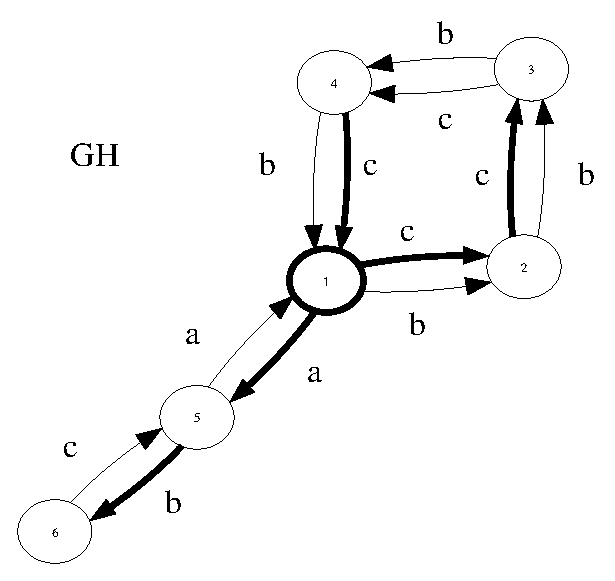
\includegraphics[scale=.5]{relt.eps}
\caption{}\label{fig:reltrana}
\end{subfigure}
\hspace{25mm}
\begin{subfigure}[b]{.45\columnwidth}
\psfrag{5-3}{\scriptsize$(5,3)$}
\psfrag{6-4}{\scriptsize$(6,4)$}
\psfrag{1-5}{\scriptsize$(1,5)$}
\psfrag{3-5}{\scriptsize$(3,5)$}
\psfrag{4-6}{\scriptsize$(4,6)$}
\psfrag{2-6}{\scriptsize$(2,6)$}
\psfrag{6-2}{\scriptsize$(6,2)$}
\psfrag{5-1}{\scriptsize$(5,1)$}
\psfrag{a}{$a$}
\psfrag{b}{$b$}
\psfrag{c}{$c$}
\psfrag{GHa}{$\G_{H_a}$}
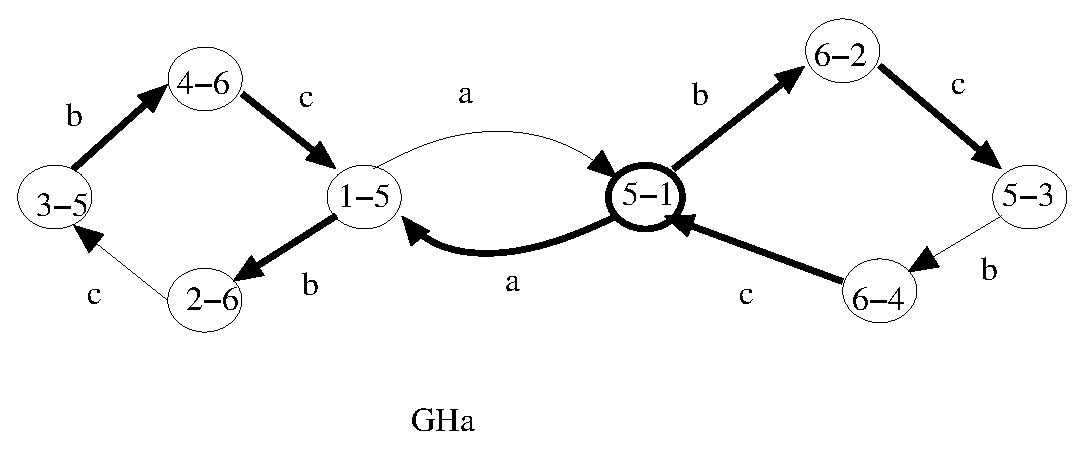
\includegraphics[scale=.7]{reltd.eps}
\caption{}\label{fig:reltranb}
\end{subfigure}
\end{center}
\caption{}\label{fig:reltran}
\end{figure}
%%%%%%%%%%%%%%%%%%%%% 
\begin{comment}
\begin{theorem}\label{thm:dcnf} Let $D_1$ and $D_2$ be sets of  double coset representatives for
$H_1\le F_1$ and $H_2\le F_2$, respectively. 
Then every element of $G$ is represented by a unique element of
$\FF(X_1\cup X_2\cup Z)$ in double coset normal form, with respect
to $D_1\cup D_2$.
\end{theorem}
\begin{proof}
To see that every $g\in G$ can be written in dc-normal form, first
write $g$ in reduced form. If the reduced form of $g$ is the empty
word then this is also the dc-normal form; with $k=0$ and $h_0=1$. 
Otherwise we have $g=f_1\cdots f_t$, where $f_i$ is in $F_{j_i}$, for
$j_i\in \{1,2\}$. In this case, let $a_is_ib_i$
be the double coset representative of $f_i$, where 
$a_i,b_i\in H_{j_i}$ and $s_i\in D_{j_i}$. For $i=1,\ldots ,t$,
 let $z^{\prime}_i=\phi_j^{-1}(a_i)$ and
$z^{\prime\prime}_i=\phi_j^{-1}(b_i)$. For $i=1,\ldots ,t-1$, let 
$z_i$ be the free reduction of $z^{\prime}_iz^{\prime\prime}_{i+1}$, 
and let $z_0=z^{\prime}_1$ and $z_t=
z^{\prime\prime}_t$. 
 If $t=1$ and $f_1\in H_{j_1}$ then $a_1=f_1$, $s_1=1$, $b_1=1$ and 
the dc-normal form of $g$ is $z_0$. Otherwise, for all $i\ge 1$, we 
have $f_i\notin H_1\cup H_2$, so $s_i\neq 1$ and 
\[z_0s_1z_1\cdots z_{t-1}s_tz_t\]
is a dc-normal form for $g$.

Now suppose that $w$ and $w^\prime$ are words in dc-normal form and that
$w=_G w^\prime$. We show by induction on $k$ that $w=w'$. 
Let $w=h_{0}p_1h_{1}p_2 \cdots h_{k-1}p_kh_{{k}}$,
and $w^\prime =h_{0}^\prime p_1^\prime h_{1}^\prime  p_2^\prime
\cdots h_{k-1}^\prime p_k^\prime h_{{k^\prime}}^\prime$, where
$h_i, h_i^\prime\in \FF(Z)$ and $p_i,p_i^\prime\in D_1\cup D_2$.
%If $w$ is the empty word then $k=0$ and $h_0=1$ and in this case it follows
%from \cite[Chapter IV, Theorem 2.6]{LS} that $k'=0$ and $h'_0=1$, so 
%$w=w'$. Hence we  assume that either $k>0$ or $h_0\neq 1$. 
If $k=0$ let $f_1=\phi_1(h_0)$ and, if $k>0$, 
let $f_1=\phi_{j_1}(h_0)p_1\phi_{j_1}(h_1)$, where $p_1\in F_{j_1}$. 
 In addition, if $k>0$,  
 for fixed $i\ge 2$, assuming that $p_i\in F_{j_i}$, 
let $f_i=p_i\phi_{j_i}(h_i)$.
 Then $f_1\cdots f_k$, is
a reduced form for the element $w\in G$. Similarly, we obtain a reduced
form $f_1^\prime \cdots f_{k^\prime}^\prime$ for $w^\prime=_G w$. 

If $k=0$ then we have $w=_G f_1=\phi_1(h_0)\in H_{1}$, and since all 
reduced forms representing an element have the same length, $k'=0$ or $1$. 
Moreover, as $f'_1=_G w\in H_1$ we have 
 $k^\prime =0$ and $w^\prime=_G f_1^\prime=\phi_1(h_0^\prime)\in H_1$.
As $H_1$ embeds in $G$ this implies that $\phi_1(h_0)=\phi_1(h'_0)$, so
$w=h_0=h'_0=w'$. Thus the result
holds when $k=0$ and we may assume inductively that $k>0$ and the result holds
for elements represented by normal forms of length less than $k$.

Comparing the lengths of reduced forms, we have $k=k^\prime$.
Moreover, $1=_G w^\prime w^{-1}= f_1^\prime \cdots f_{k}^\prime
f_k^{-1}\cdots f_1^{-1}$, so by \cite[Chapter IV, Theorem 2.6]{LS}, 
we have $ f_{k}^\prime f_k^{-1}\in H_{j_k}$, where $j_k=1$, or $2$. Hence, for
some $a, b\in H_{j_k}$ we have $p_k^\prime=a p_k b$. Therefore $p_k^\prime =p_k$,
and now, as $p_k$ is a double coset representative and  $ f_{k}^\prime f_k^{-1}\in H_{j_k}$,
it follows that $h_k=h_k^\prime$. Hence $f_1\cdots f_{k-1}=
f_1^\prime \cdots f_{k-1}^\prime$ and, applying the inductive hypothesis,
  we see that $w=w^\prime$, as required.
\end{proof}
\end{comment} 
%%%%%%%%%%%%%%%%%%%%%%%%%%%%%%%%%%%
~\\[1em]

\noindent\textbf{Algorithm III}. \\

\ajd{This is the version with $Z$ components.}\\
Here each step of the algorithm is described and shown to preserve the image of the map $\pi:L \maps G$.
A  
summary of the algorithm is given in Section \ref{sub:summaryIII}.  
Let $\D$ be an inverse automaton, with alphabet $\S$ and
start and final state $1$, such that
$\pi(L(\D))=K$.
For $k=1,2$, let $\D_k$ be the graph formed from $\D$ by removing all edges of
type $X_{k^\prime}$, where $k\neq k^\prime$. An $X_k$ component of
$\D_k$ is the subgraph of $\D$, containing at least one edge of type $X_k$, 
 formed from a connected component
of $\D_k$ by removing all leaves which are incident to edges of
type $Z$, and then repeating the process till there are no such
leaves left. Given an $X_k$ component $\T$ of $\D_k$,  a
{\em boundary vertex} of $\T$ is defined to be a vertex
$\a$ such that $\a$ is incident, in $\D$, to a vertex which does not
belong to $\T$.
 We shall modify each  $X_k$ component $\T$ of $\D_k$ so that if $p$ is a path,
from a  boundary vertex $u$  to a boundary vertex $v$ of $\T$,
then the normal form  of  the label $l(p)$ of $p$ is the label of
a path from $u$ to $v$. Throughout the modification process we
keep track of the boundary vertices, so that once modification is
complete the $X_k$ components can be reassembled, by attaching as
they did in $\D$. The modification of an $X_k$ component $\Theta$
of $\D_k$ consists of
five steps, producing new graphs $\T_1$, $\T_2$, $\T_3$, $\T_4$
and $\T_5$. In each case there is a canonical morphism $\theta_i$
from $\T_{i-1}$ to $\T_i$ and,
 (writing $\T=\T_0$)
we define the {\em boundary vertices} of $\T_{i}$ to be the vertices $\theta_{i}(v)$
of $\T_i$, such that $v$ is a boundary vertex of $\T_{i-1}$. Moreover the
 images $\theta_i\circ \cdots\circ \theta_1(v)$ of vertices of $\T$ in $\T_i$
will be referred to as  {\em vertices of} $\T$.


The modification process is followed by a ``reassembly'' phase, in which
we reconnect the $X_k$ components of $\D$, 
to form the output of the algorithm. 
To enable the reassembly the algorithm records, when constructing 
$\Theta_{i}$ from $\Theta_{i-1}$, the inverse images of vertices of 
$\Theta_{i}$ under the map $\theta_i$. We leave details of the
construction of these inverse image sets to the the summary
in 
Section \ref{sub:summaryIII}. 
 
Let $\T$ be an $X_k$ component of $\D_k$.
\\[1em]
%%%%%%%%%%%%%%%%%%%%%%%%%%%%%%
\ajd{This is the ``$\D_Z$ version'' of Step \ref{it:D1} of alg III.}
\be
\item\label{it:D1a} Remove all edges of type $X_{k'}$, where $k'=3-k$, from $\D$ to give a graph $\D'_{k,0}$.
\item\label{it:D1b} A \emph{shoot} is an edge incident to a leaf. Remove all shoots
of type $Z$ from $\D'_{k,0}$; adding
edges removed to  a graph $\D_Z$ (which starts off empty, when $k=1$, and 
is not reinitialised when $k$ is incremented to $2$). Continue
until there are no shoots of type $Z$ in $\D'_{k,0}$. The resulting graph
is $\D_{k,0}$. 
\item\label{it:D1c} Rename vertices of $\D_{k,0}$: 
a vertex named $v$ in $\D$ becomes
$(v,k)$ in $\D_{k,0}$.
\item\label{it:D1d} For each vertex $(v,k)$ of $\D_{k,0}$,  set 
  $\vim(v,k)$ equal to $\{v\}$.  For each vertex $v$ of $\D_Z$, 
set $\vim(v)=\{v\}$. 
\ee
~\\[1em]
\ajd{This is the ``$\D_Z$ version'' of Reassemby.}
\item\label{it:D16.5} Set $\D'_5$ equal to the disjoint union
$\D_{1,5}\cup \D_{2,5}\cup \D_Z$. 
\item\label{it:D17} (\textbf{Begin Reassembly}.) 
For each vertex $(u,k)$ of $\D_{1,5}\cup \D_{2,5}$,
do the following. For each vertex $(v,k')$ of $\D_{1,5}\cup \D_{2,5}$, not
equal to $(u,k)$, if
$\vim((u,k))\cap \vim((v,k'))\neq \emptyset$ then replace  
$\vim((u,k))$ with $\vim((u,k))\cup
\vim((v,k'))$. In this case, for each edge $e$ of $\D_{1,5}\cup \D_{2,5}$, if $e$ has
initial or terminal vertex equal to $(v,k')$ then replace $e$ with
an edge having $(u,k)$ as initial or terminal vertex, instead of $(v,k')$.
Delete $(v,k')$, once no more such edges exist.
Continue for as long as possible: that is until 
$\vim(u,k)\cap \vim(u',k')=\emptyset$, whenever $(u,k)\neq (u',k')$. The resulting graph is denoted $\D''_5$.
\item\label{it:D18} 
If $\a\in \vim(u,k)$, 
%If $\vim(\a)\cap \vim(u,k)\neq \nul$,
 for some
 vertices $\a$ of $\D_Z$ and $(u,k)$ of $\D''_5$ then replace $\a$ 
with $(u,k)$. % and add $\a$ to $\vim(u,k)$. 
(Note that, as
we have completed step \ref{it:D17}, there is at most one such vertex of
$\D'_5$.)
If $\a$ has been replaced by $(u,k)$ then, for every edge $e$ of $\D_Z$,
 of the form $(\a,\b)$ (or its reverse), replace $e$ with
 the edge $((u,k), \b)$ (or its reverse). Call the resulting graph $\D_Z''$.
\item\label{it:D19} Form $\D''$ from the union of $\D''_5$ and $\D_Z''$:
 by identifying vertices of $\D_Z''$ with vertices of  $\D''_5$
of the same name.
%\item\label{it:D20}  Construct $\D''$, the Stallings folding of $\bar \D$.
\ee
In Lemma \ref{lem:idverts} below we verify that the graph output from 
Step \ref{it:D19} is the same as the graph $\D''$ constructed in Section
\ref{sec:dca}, using the equivalence relation $\approx$.  

\end{document}